% Options for packages loaded elsewhere
\PassOptionsToPackage{unicode}{hyperref}
\PassOptionsToPackage{hyphens}{url}
\PassOptionsToPackage{dvipsnames,svgnames,x11names}{xcolor}
%
\documentclass[
  11pt,
]{article}
\usepackage{amsmath,amssymb}
\usepackage{iftex}
\ifPDFTeX
  \usepackage[T1]{fontenc}
  \usepackage[utf8]{inputenc}
  \usepackage{textcomp} % provide euro and other symbols
\else % if luatex or xetex
  \usepackage{unicode-math} % this also loads fontspec
  \defaultfontfeatures{Scale=MatchLowercase}
  \defaultfontfeatures[\rmfamily]{Ligatures=TeX,Scale=1}
\fi
\usepackage{lmodern}
\ifPDFTeX\else
  % xetex/luatex font selection
\fi
% Use upquote if available, for straight quotes in verbatim environments
\IfFileExists{upquote.sty}{\usepackage{upquote}}{}
\IfFileExists{microtype.sty}{% use microtype if available
  \usepackage[]{microtype}
  \UseMicrotypeSet[protrusion]{basicmath} % disable protrusion for tt fonts
}{}
\makeatletter
\@ifundefined{KOMAClassName}{% if non-KOMA class
  \IfFileExists{parskip.sty}{%
    \usepackage{parskip}
  }{% else
    \setlength{\parindent}{0pt}
    \setlength{\parskip}{6pt plus 2pt minus 1pt}}
}{% if KOMA class
  \KOMAoptions{parskip=half}}
\makeatother
\usepackage{xcolor}
\usepackage[margin=1in]{geometry}
\usepackage{longtable,booktabs,array}
\usepackage{calc} % for calculating minipage widths
% Correct order of tables after \paragraph or \subparagraph
\usepackage{etoolbox}
\makeatletter
\patchcmd\longtable{\par}{\if@noskipsec\mbox{}\fi\par}{}{}
\makeatother
% Allow footnotes in longtable head/foot
\IfFileExists{footnotehyper.sty}{\usepackage{footnotehyper}}{\usepackage{footnote}}
\makesavenoteenv{longtable}
\usepackage{graphicx}
\makeatletter
\def\maxwidth{\ifdim\Gin@nat@width>\linewidth\linewidth\else\Gin@nat@width\fi}
\def\maxheight{\ifdim\Gin@nat@height>\textheight\textheight\else\Gin@nat@height\fi}
\makeatother
% Scale images if necessary, so that they will not overflow the page
% margins by default, and it is still possible to overwrite the defaults
% using explicit options in \includegraphics[width, height, ...]{}
\setkeys{Gin}{width=\maxwidth,height=\maxheight,keepaspectratio}
% Set default figure placement to htbp
\makeatletter
\def\fps@figure{htbp}
\makeatother
\setlength{\emergencystretch}{3em} % prevent overfull lines
\providecommand{\tightlist}{%
  \setlength{\itemsep}{0pt}\setlength{\parskip}{0pt}}
\setcounter{secnumdepth}{-\maxdimen} % remove section numbering
\ifLuaTeX
  \usepackage{selnolig}  % disable illegal ligatures
\fi
\IfFileExists{bookmark.sty}{\usepackage{bookmark}}{\usepackage{hyperref}}
\IfFileExists{xurl.sty}{\usepackage{xurl}}{} % add URL line breaks if available
\urlstyle{same}
\hypersetup{
  pdfauthor={Stefano Alimonti --- stefalimonti@gmail.com},
  colorlinks=true,
  linkcolor={blue},
  filecolor={Maroon},
  citecolor={Blue},
  urlcolor={blue},
  pdfcreator={LaTeX via pandoc}}

\author{Stefano Alimonti --- stefalimonti@gmail.com}
\date{March 2026}

\begin{document}

{
\hypersetup{linkcolor=black}
\setcounter{tocdepth}{2}
\tableofcontents
}
\section{Reader's Guide: The Trace Anomaly of Binary
Multiplication}\label{readers-guide-the-trace-anomaly-of-binary-multiplication}

\textbf{Stefano Alimonti} --- March 2026

\emph{This guide summarizes the analytical mechanism by which π enters the
sector ratio of binary multiplication. It assumes familiarity with the basic
setup (carries, D-odd products, sectors) as presented in {[}P1, Reader's
Guide{]}.}

\begin{center}\rule{0.5\linewidth}{0.5pt}\end{center}

\newpage

\subsection{1. The Decomposition R = R₀ +
ΔR}\label{the-decomposition-r-rux2080-ux3b4r}

The sector ratio \(R(K)\) --- the carry-weighted ratio of D-odd pairs in sectors
(1,0) and (0,0) --- can be computed by two different ``readout'' methods:

\begin{itemize}
\tightlist
\item
  \textbf{Schoolbook:} Read the carry at the fixed position \(L - 2\)
  (second-highest carry). This gives a ratio \(R_0 = -3.931205\ldots\), a purely
  logarithmic constant involving only \(\ln 2\) and \(\ln 3\).
\item
  \textbf{Cascade:} Scan downward from the top, stop at the first nonzero carry,
  and read one position below. Numerically, this gives strong evidence for
  \(R \to -\pi = -3.14159\ldots\).
\end{itemize}

The difference \(\Delta R = R - R_0 = +0.790\ldots\) is where all the
transcendental content lives. The schoolbook limit is proved (Proposition 1);
the cascade correction is where the mystery lies.

\begin{center}\rule{0.5\linewidth}{0.5pt}\end{center}

\newpage

\subsection{2. The Linear Mix Hypothesis
(LMH)}\label{the-linear-mix-hypothesis-lmh}

The paper proposes a specific mechanism: the effective carry transfer operator
decomposes as

\[\mathcal{K}_{\mathrm{eff}} = (1-A) \cdot \mathcal{K}_{\mathrm{Markov}} + \frac{A}{2} \cdot I\]

where \(\mathcal{K}_{\mathrm{Markov}}\) is the independent-carry (Markov)
operator and \(A > 1\) is a scalar parameter measuring the strength of digit
correlations. This is a ``linear mix'' of the Markov operator with a pure-noise
term.

Under the LMH, the effective eigenvalues of the carry bridge become

\[\lambda_n^{\mathrm{eff}} = (1 - A) \cdot \frac{1}{2}\cos\!\left(\frac{n\pi}{L}\right) + \frac{A}{2}\]

and the corresponding effective spectral sum is the closed-form Möbius
transformation

\[S(A) = \frac{2(1-A)}{3-2A}\]

proved in {[}P1, Theorem 1{]}. If the physical cascade ratio is governed by the
LMH/resolvent-universality model of {[}E{]}, this identifies the observed sector
ratio with \(S(A)\).

\begin{center}\rule{0.5\linewidth}{0.5pt}\end{center}

\newpage

\subsection{3. The Phase Transition}\label{the-phase-transition}

\begin{longtable}[]{@{}lll@{}}
\toprule\noalign{}
\(A\) & \(S(A)\) & Interpretation \\
\midrule\noalign{}
\endhead
\bottomrule\noalign{}
\endlastfoot
0 & +2/3 & Markov (no correlations): rational, positive \\
1 & 0 & Critical point: exact cancellation \\
\(A^* \approx 1.379\) & \(-\pi\) & LMH value matching the observed limit \\
3/2 & \(\pm\infty\) & Pole (divergence) \\
\end{longtable}

Within the LMH model, as digit correlations increase from \(A = 0\) to \(A^*\),
the spectral sum crosses zero and reaches \(-\pi\). This places the model at
distance \(1/(2(\pi + 1)) \approx 0.121\) from the pole --- remarkably close to
divergence.

\begin{figure}
\centering
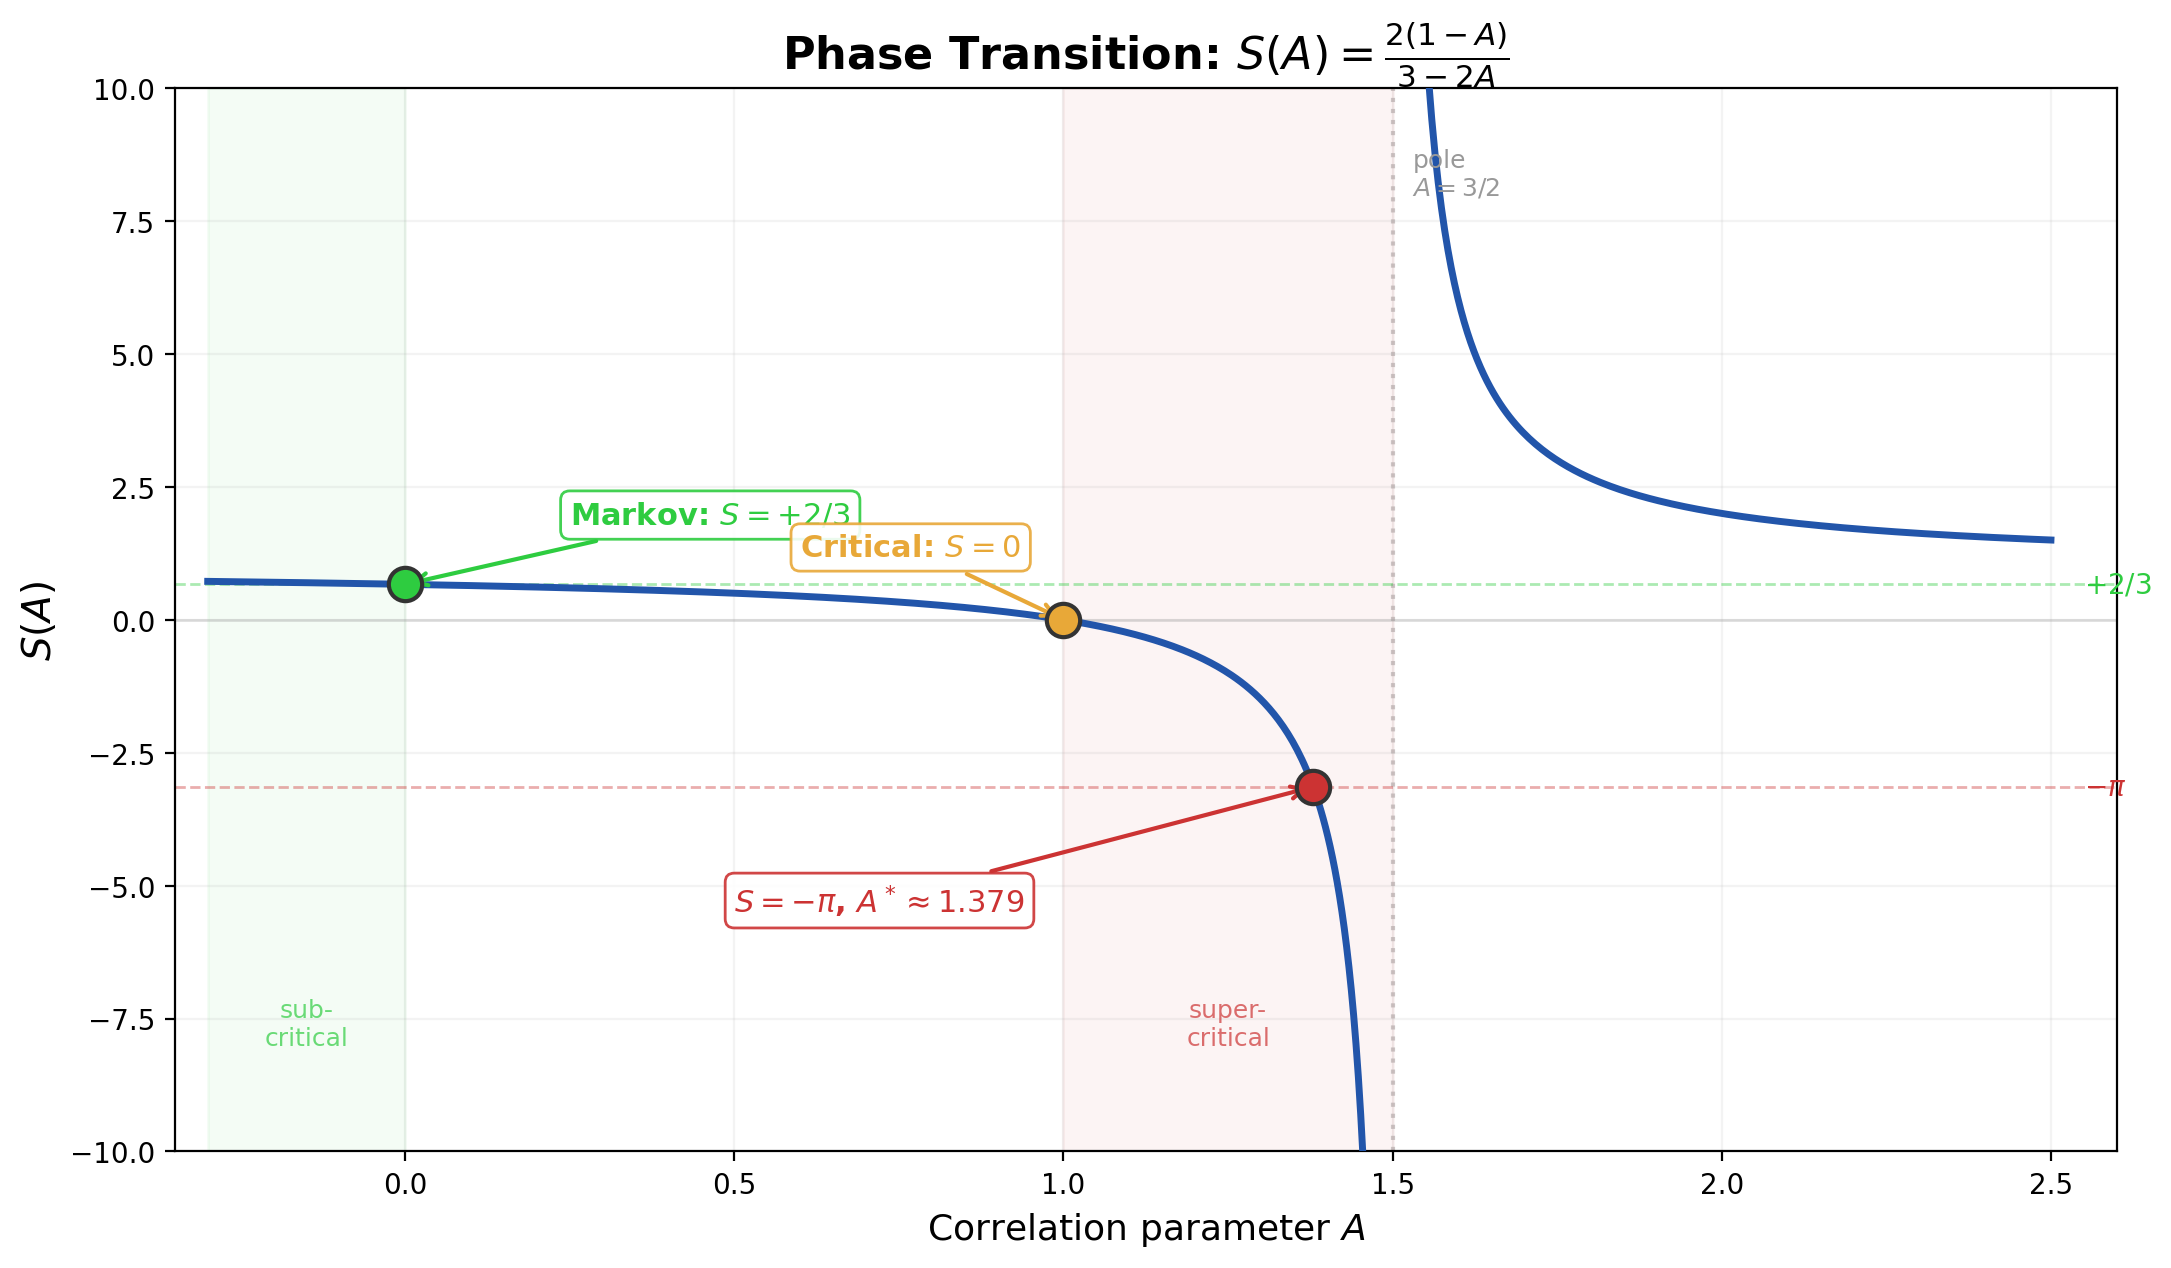
\includegraphics{../figures/fig_phase_transition.png}
\caption{Phase transition: S(A) Möbius curve}
\end{figure}

\begin{center}\rule{0.5\linewidth}{0.5pt}\end{center}

\newpage

\subsection{4. Three Falsification Results}\label{three-falsification-results}

To test the LMH against the main alternatives, the paper systematically
falsifies several competing explanations:

\textbf{Falsification 1 (Boundary geometry).} If \(\pi\) came from the D-parity
boundary curve \(\alpha + \beta = \pi/4\) {[}G{]}, it should be localized in
pairs near the boundary. Decomposing contributions by boundary proximity
(through depth 12) shows that \(\pi\) is \emph{not} concentrated at the boundary
--- it is distributed across the full domain (Observation 2).

\textbf{Falsification 2 (Critical cell area).} The cell where the cascade
correction \(\Delta R\) peaks has area \(-3/16 + 7/4 \cdot \ln(28/25)\), a
rational combination of logarithms with no \(\pi\) (Proposition 3). The
transcendental content enters through the \emph{weighting} of cells, not their
geometry.

\textbf{Falsification 3 (Generic operators).} No diagonal perturbation of a
cosine-spectrum operator can reproduce the Linear Mix --- the trace obstruction
prevents it (Observation 4). The LMH requires a specific off-diagonal structure
that mirrors the Diaconis-Fulman carry dynamics.

\begin{center}\rule{0.5\linewidth}{0.5pt}\end{center}

\newpage

\subsection{5. The Resolvent Universality
Mechanism}\label{the-resolvent-universality-mechanism}

Under the LMH/resolvent-universality model, the relevant spectral sum is taken
over the Dirichlet eigenmodes of the carry bridge. In the \(L \to \infty\)
limit, the spectral weights \(\sin(n\pi/2)\) (for \(n \geq 1\)) coincide with
the Dirichlet character \(\chi_4(n) = (1, 0, -1, 0, 1, 0, -1, \ldots)\)
restricted to the odd modes \(n = 1, 3, 5, \ldots\) that carry the alternating
sign. The resulting sum

\[\sum_{k=0}^{\infty} \frac{(-1)^k}{1/2 + \beta \sin^2((2k+1)\pi/(2L))}\]

converges to \(2\beta/(1 + 2\beta)\) (proved). Choosing
\(\beta = -\pi/(2+2\pi)\), equivalently \(A = A^*\), makes this model sum equal
to \(-\pi\).

The key insight: no single Fourier mode carries the \(\pi\)-content. Instead,
the \textbf{resolvent} --- the inverse \((I - \lambda T)^{-1}\) of the transfer
operator --- redistributes the spectral weight collectively. In the proposed
universality mechanism, \(-\pi\) emerges from the \emph{collective behavior} of
all modes, not from any individual one.

\begin{center}\rule{0.5\linewidth}{0.5pt}\end{center}

\newpage

\subsection{6. What Remains Open}\label{what-remains-open}

The paper leaves two explicit closure points in the proposed
LMH/resolvent-universality mechanism:

\begin{enumerate}
\def\labelenumi{\arabic{enumi}.}
\item
  \textbf{The effective \(\chi_4\)-channel closure:} Prove that the
  LMH/resolvent-universality mechanism fixes the effective \(\chi_4\)-channel
  constant so that the model sum matches \(-\pi\) (equivalently, the closure
  corresponding to \(A = A^*\)).
\item
  \textbf{Spectral gap preservation:} Prove that the Diaconis-Fulman spectral
  gap \(\rho = 1/2\) is preserved when the carry chain is conditioned on the
  D-odd constraint (\(c_0 = c_L = 0\)).
\end{enumerate}

Both are analytically tractable targets. The first now has a precise
operator-side formulation in {[}L{]}: the mixed stopping-time channel is
realized as a canonical weighted first-return resolvent and its \(s=1\) closure
reduces to a scalar \texttt{χ₄\ -\textgreater{}\ L(1,\textbackslash{}chi\_4)}
constant. The second requires a perturbation argument for the
boundary-conditioned transfer operator. The same companion analysis shows that
the present carry-side object remains zero-free in the tested strip box and does
not admit a simple gamma-like completion there, so the missing ingredient is not
another fit but a genuine phase/completion mechanism.

\begin{center}\rule{0.5\linewidth}{0.5pt}\end{center}

\newpage

\subsection{References}\label{references}

\begin{enumerate}
\def\labelenumi{\arabic{enumi}.}
\tightlist
\item
  {[}P1{]} S. Alimonti, ``π from Pure Arithmetic: A Spectral Phase Transition in
  the Binary Carry Bridge,'' this series.
  doi:\href{https://doi.org/10.5281/zenodo.18895611}{10.5281/zenodo.18895611}
  ---
  \href{https://github.com/stefanoalimonti/carry-arithmetic-P1-pi-spectral}{GitHub}
\item
  {[}A{]} S. Alimonti, ``Spectral Theory of Carries in Positional
  Multiplication,'' this series.
  doi:\href{https://doi.org/10.5281/zenodo.18895593}{10.5281/zenodo.18895593}
  ---
  \href{https://github.com/stefanoalimonti/carry-arithmetic-A-spectral-theory}{GitHub}
\item
  {[}G{]} S. Alimonti, ``The Angular Uniqueness of Base 2 in Positional
  Multiplication,'' this series.
  doi:\href{https://doi.org/10.5281/zenodo.18895601}{10.5281/zenodo.18895601}
  ---
  \href{https://github.com/stefanoalimonti/carry-arithmetic-G-angular-uniqueness}{GitHub}
\item
  {[}L{]} S. Alimonti, ``The Carry--Dirichlet Bridge: Stopping-Time Series and
  L²(s,χ₄),'' this series.
  doi:\href{https://doi.org/10.5281/zenodo.18895609}{10.5281/zenodo.18895609}
  ---
  \href{https://github.com/stefanoalimonti/carry-arithmetic-L-dirichlet-bridge}{GitHub}
\end{enumerate}

\begin{center}\rule{0.5\linewidth}{0.5pt}\end{center}

\emph{CC BY 4.0}

\end{document}
